\chapter{Termo de Abertura do projeto}

\section{EAP}
\section{Lista É/Não é}
\subsection{É}
\subsection{Não é}
\section{Requisitos}
\subsection{Eletrônica}
\subsection{Energia}
\subsection{Estrutura}


Os requisitos a serem considerados na elabora\c c\~ao e projeto estrutural dever\~ao considerar principalmente as condi\c c\~oes clim\'aticas da regi\~ao (esta\c c\~oes do ano, varia\c c\~ao de umidade e temperatura, velocidade m\'axima do vento e poss\'iveis fatores locais que possam interferir ou no funcionamento da estrutura ou no funcionamento dos componentes eletr\^onicos), al\'em das cargas geradas pelos próprios componentes estruturais. Para isso, foi realizada uma pesquisa em sites de metereologia que pudessem fornecer as informa\c c\~oes clim\'aticas da regi\~ao de Serra, onde as informações fornecidas foram retiradas do site de meteorologia do estado do Esp\'irito Santo.
A regi\~ao da Serra, de forma ampla, fica no estado do Esp\'irito Santo, na regi\~ao sudeste do Brasil, localizado na Microrregi\~ao de Vit\'oria e na Mesorregi\~ao Central Esp\'irito-Santense, como pode ser observado em \ref{mapa_es}. O clima predominante da regi\~ao sudeste litor\^anea do Brasil \'e o Tropical Atl\^antico (tropical \'umido), que apresenta grande influ\^encia da umidade vinda do Oceano Atl\^antico. As caracter\'isticas desse tipo de clima s\~ao: temperaturas elevadas no ver\~ao (podendo atingir at\'e 40$^\circ$C) e amenas no inverno (m\'edia de 20$^\circ$C), e em fun\c c\~ao da umidade trazida pelo oceano, costuma chover muito nestas \'areas.

Os dados trazidos aqui são referentes às análises estátisticas de relatórios horários adquiridos entre janeiro de 1980 e dezembro de 2016. 


\begin{figure}[H]
	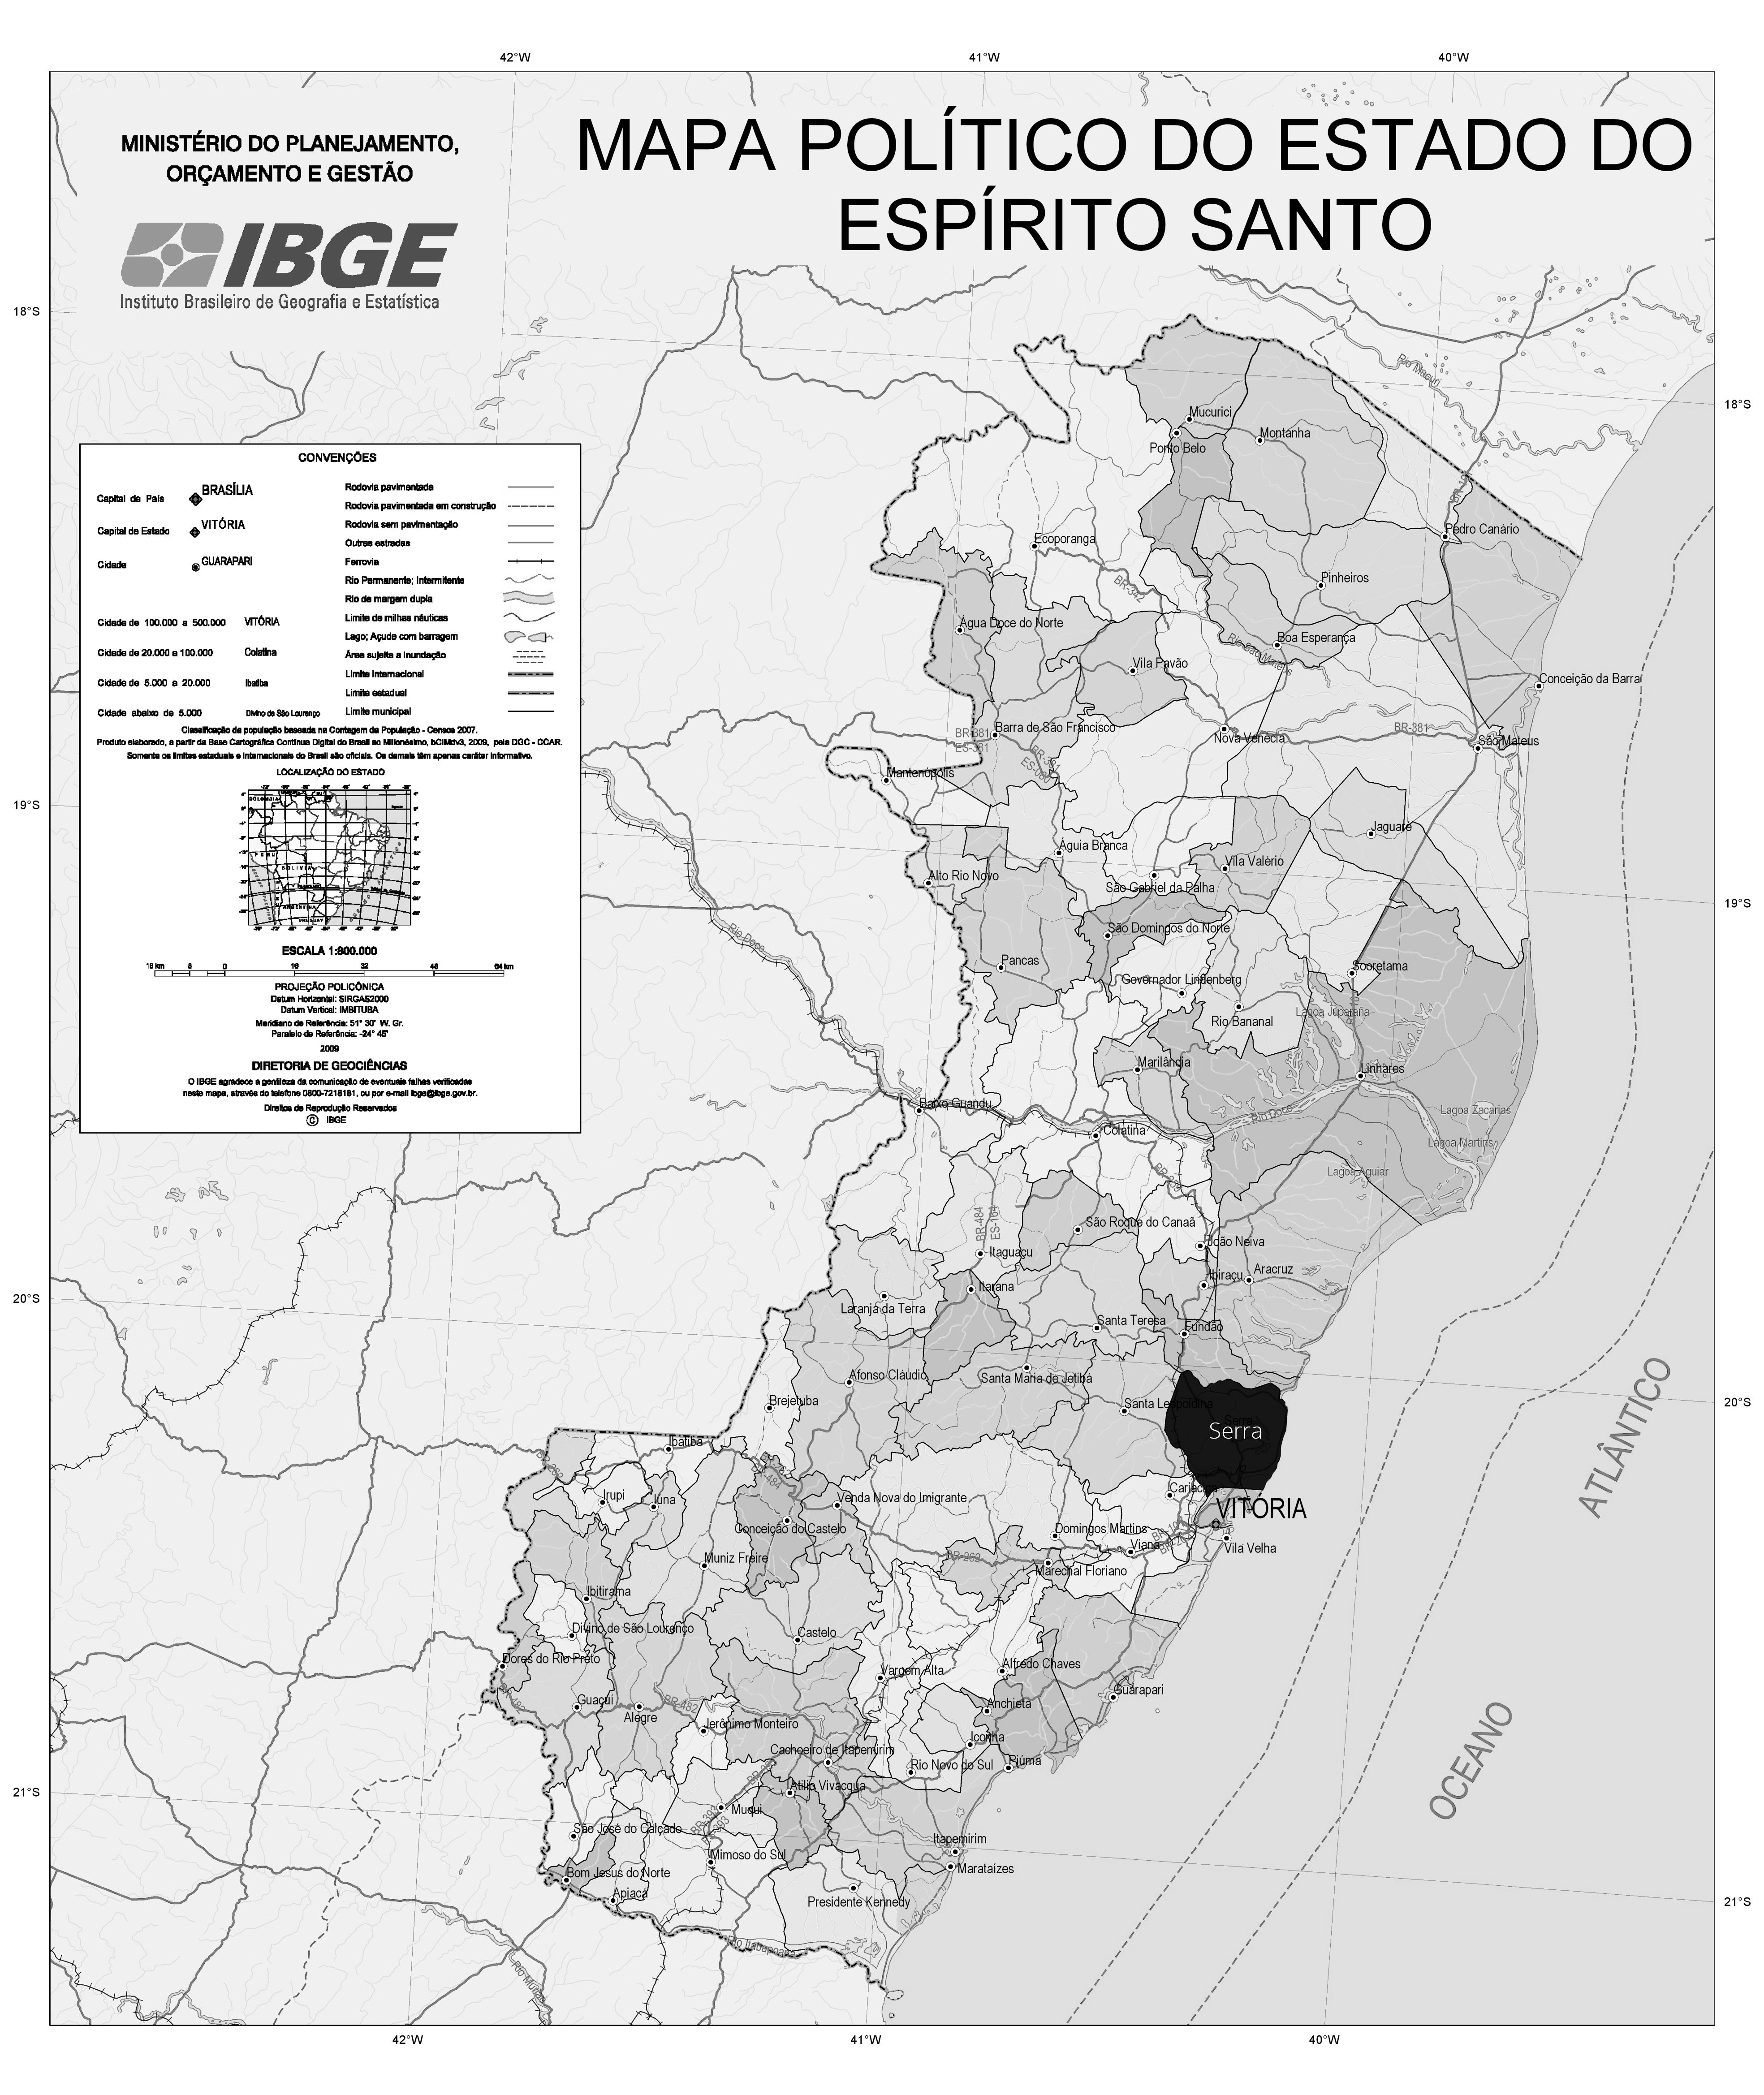
\includegraphics[scale=0.2]{mapa_es.png}
	\centering
	\caption{Mapa regional do Estado do Espírito Santo}
	\label{mapa_es}
	
\end{figure}

Dessa forma, o clima do município de Serra é dividido da seguinte maneira:

\begin{figure}[!htb]
	\includegraphics[scale=0.8]{reg_serra.png}
	\centering
	\caption{Zonas naturais da região de Serra. Fonte: Zonas Naturais do Espírito Santo (EMCAPA/NEPUT (1999))}
	\label{regiao_serra}
\end{figure}

\begin{figure}
	\includegraphics[scale=1]{tabela_serra}
	\centering
\end{figure}

Será considerado de forma majoritária a climatização da zona 8, por ocupar uma maior porcentagem de área na região.
Assim, foram pesquisadas de forma mais a fundo os valores médios das características climáticas da região (analisadas entre os anos de 1980 e 2016 segundo Y), tais como temperatura, nuvens, precipitação, chuva, Sol, umidade, ventos e energia solar incidente apresentados abaixo. Vale  

\subsubsection{Temperatura}

\begin{figure}[H]
	\includegraphics[scale=1]{mapa_temp}
	\centering
	\caption{Gráfico de temperatura média na região de Serra - ES.}
\end{figure}

Para o gráfico de temperaturas, é possível observar que durante o verão, a temperatura média mais alta é de 32º, enquanto durante o inverno, a mínima média é de 18º. 

\begin{figure}[H]
	\includegraphics[scale=1]{mapa_temp2}
	\centering
	\caption{Gráfico de temperatura média horária na região de Serra - ES.}
\end{figure}

A análise gráfica dos daods de precipitação, chuva mensal e umidade severão ser analisados juntos para uma melhor interpretação pois eles se complementam.

\subsubsection{Precipitação}

\begin{figure}[H]
	\includegraphics[scale=1]{mapa_prep}
	\centering
	\caption{Gráfico de precipitação média na região de Serra - ES.}
	\label{mapa_prep}
\end{figure}

\subsubsection{Chuva}
\begin{figure}[H]
	\includegraphics[scale=1]{mapa_chuva}
	\centering
	\caption{Gráfico das chuvas médias na região de Serra - ES.}
	\label{mapa_chuva}
\end{figure}
\subsubsection{Umidade}
\begin{figure}[H]
	\includegraphics[scale=1]{mapa_umidade}
	\centering
	\caption{Gráfico da umidade média na região de Serra - ES.}
	\label{mapa_umidade}
\end{figure}

Análisando os gráficos \ref{mapa_prep}, \ref{mapa_chuva}, \ref{mapa_umidade} é possível relacioná-los em relação as épocas de seca e umidade, além de poder ser possível observar que os períodos quando ocorrem serem no inverno (baixas temperaturas) e verão (altas temperaturas), respectivamente. Essa análise é importante, pois além de ser necessário escolher um material que seja resistente tanto a condições de seca como de umidade, é necessário escolher um material que seja resistente à essas variações de temperatura mas que também seja ao contato constante com a chuva e umidade. Sabe-se que climas secos estão relacionados à uma variação de temperatura mais rápida entre as temperaturas máxima e mínima, enquanto dias úmidos estão relacionados à uma variação mais lenta.
 
\subsubsection{Velocidade do vento}

\begin{figure}[H]
	\includegraphics[scale=1]{velocidade_vento}
	\centering
	\caption{Gráfico develocidade média do vento na região de Serra - ES.}
	\label{vel_vento}
\end{figure}

Um fator mecânico importante a ser analisado é a velocidade do vento na estrutura, pois ele é responsável por esforços mecânicos que a estrutura terá que resistir. Pode-se analisar o gráfico \ref{vel_vento} e perceber que ele traz valores médios para a velocidade do mesmo. Entretanto, a fim de projetar-se uma estrutura que seja eficiente é necessário analisar a valocidade máxima do vento nos períodos de ventos fortes. Para isso, analisou-se o dia 07 de outubro que trouxe uma velocidade média acima das demais:

\begin{figure}[H]
	\includegraphics[scale=1]{velocidade_vento_dia07}
	\centering
	\caption{Gráfico de velocidade média do vento no dia 07 de outubro na região de Serra - ES.}
\end{figure}

Analisando as velocidades médias do vento no dia 07, vê-se que a velocidade máxima do mesmo neste dia foi de 21 Km/h. Dessa forma, é necessário perceber as variações de fatores importantes que possam interferir na eficiencia estrutural do projeto e traze-los para o projeto de forma a ter uma estrutura resistente.


\subsubsection{Incidência solar}


\begin{figure}[H]
	\includegraphics[scale=1]{mapa_inci_solar}
	\centering
	\caption{Gráfico da incidencia solar média nna região de Serra - ES.}
\end{figure}

É necessária uma análise da indicência solar na região levando em consideração as variações sazonais da mesma. A incidência solar é importante para o projeto em dois aspéctos: primeiro para que seja possível pesquisar materiais que sejam resistentes às ações das radiações  visíveis e também às radiações ultravioletas e, em segundo, para que seja possível fazer o projeto da placa solar que estará no topo do radar.

\subsubsection{Materiais}

O grande desafio estrutural desse projeto é conseguir aliar materiais com boas propriedades mecânicas mas que não interfiram na recepção e nem na emissão dos sinais dos componentes eletrônicos, além disso, será necessário também uma estrutura que proteja e isole os componentes eletrônicos das ações climáticas da região. 

\subsubsection{Manutenção}

É necessário projetar uma estrutura que permita o acesso de técnicos de forma segura, eficiente e rápida para manutenções periódicas (ou quando necessárias) por se tratar de um projeto que tem como áreas de atuação e instalação estradas de alta velocidade e serras.

\subsection{Software}
\section{\emph{Stakeholders}}
\section{Recurso humanos}
\section{Cronograma de atividades}
\section{Milestones Identificados}
\section{Estimativa de custos}
\section{Viabilidades financeira}
\section{Levantamento de riscos}
